\subsection*{Inferring the noise profile from replicate experiments} 

To study variations arising from experimental noise, we analysed replicates of repertoire sequencing experiments. The tasks of learning the noise model and the distribution of clone sizes are impossible to dissociate. To infer $P(n|f)$, one needs to get a handle on $f$, which is unobserved, and for which the prior distribution $\rho(f)$ is essential. Conversely, to learn $\rho(f)$ from the read counts $n$, we need to deconvolve the experimental noise, for which $P(n|f)$ is needed. Both can be learned simultaneously from replicate experiments (i.e. $f^\prime=f$), using maximum likelihood estimation. For each clone, the probability of observing $n$ read counts in the first replicate and $n'$ read counts in the second replicate reads:
\beq\label{eq:null}
P(n,n'|\theta_{\rm null})=\int_{f_{\rm min}}^1 \textrm{d}f\, \rho(f|\theta_{\rm null}) P(n|f,\theta_{\rm null})P(n'|f,\theta_{\rm null}),
\eeq
where $\theta_{\rm null}$ is a vector collecting all the parameters of both the noise model and the clone size distribution, namely $\theta_{\rm null}=\{f_{\rm min},\nu\}$ for the Poisson noise model, $\theta_{\rm null}=\{f_{\rm min},\nu,a,\gamma\}$ for the negative binomial noise model, and $\theta_{\rm null}=\{f_{\rm min},\nu,a,\gamma,M\}$ for the two-step noise model.

While Eq.~\ref{eq:null} gives the likelihood of a given read count pair $(n,n')$, we need to correct for the fact that we only observe pairs for which $n+n'>0$. In general,
many clones in the repertoire are small and missed in the acquisition process. In any realization, we expect $n+n'>0$ for only a relatively small number of clones, $N_{\rm obs}\ll N$. Typically, $N_{\rm obs}$ is of order $10^5$, while $N$ is unknown but probably ranges from $10^7$ for mouse to $10^8-10^{10}$ for humans \cite{Qi2014,Lythe2016}. Since we have no experimental access to the unobserved clones ($n=n^{\prime}=0$), we maximize the likelihood of the read count pairs $(n_i,n'_i)$, $i=1,\ldots,N_{\rm obs}$, conditioned on the clones appearing in the sample:
\beq\label{eq:MLE}
\hat\theta_{\rm null}=\argmax_{\theta_{\rm null}} \prod_{i=1}^{N_{\rm obs}} \frac{P(n_i,n'_i|\theta_{\rm null})}{1-P(0,0|\theta_{\rm null})}.
\eeq

While the condition $N\<f\>=1$ ensures normalization on average, we may instead require that normalization be satisfied for the particular realization of the data, by imposing:
\beq
	Z=N	P(0,0)\langle f\rangle_{\rho(f|n+n^{\prime}=0)} + \sum_{i=1}^{N_{\textrm{obs}}}\langle f\rangle_{\rho(f|n_i,n^{\prime}_i)}=1,\label{eq:postnorm}
\eeq
where $N$ is estimated as $N=N_{\textrm{obs}}/(1-P(0,0))$. The first term corresponds to the total frequency of the unseen clones, while the second term corresponds to a sum of the average posterior frequencies of the observed clones. Imposing either Eq.~\ref{eq:postnorm} or $N\<f\>=1$ yielded similar values of the parameter estimates, $\hat\theta_{\rm null}$.

%\subsubsection*{Method validation on synthetic data}

%\subsubsection*{Model validation}

To test the validity of the maximum likelihood estimator, Eq.~\ref{eq:MLE}, we created synthetic data for two replicate sequencing experiments with known parameters $\theta_{\rm null}$ under the two-step noise model, and approximately the same number of reads as in the real data.
To do so efficiently, we developed a sampling protocol that deals with the large number of unobserved clones implicitly (see Methods).
Applying the maximum likelihood estimator to these synthetic data, we correctly inferred the ground truth over a wide range of parameter choices (\cref{fig:SM_reinfer_null}).


Next, we applied the method to replicate sequencing experiments of unfractioned repertoires of 6 donors over 5 time points spanning a 1.5 month period (30 donor-day replicate pairs in total). For a typical pair of replicates, a visual comparison of the $(n,n')$ pairs generated by the Poisson and two-step noise models with the data shows that the Poisson distribution fails to explain the large observed variability between the two replicates, while the two-step model can (Fig.~\ref{fig:nullstats}A-C). The normalized log-likelihood of the two-step model was slightly but significantly higher than that of the negative binomial model, and much larger than that of the Poisson model (\cref{fig:nullstats}D). The two-step model was able to reproduce accurately the distribution of read counts $P(n)$ (Fig.~\ref{fig:modelfit}A), as well as the conditional distribution $P(n'|n)$ (Fig.~\ref{fig:modelfit}B), even though those observables were not explicitly constrained by the fitting procedure. In particular, $P(n)$ inherits the power law of the clone frequency distribution $\rho(f)$, but with deviations at low count numbers due to experimental noise, which agree with the data. 
Also, the two-step model outperformed the negative binomial noise model at describing the long tail of the read count distribution for clones that were not seen in one of the two replicates (see \cref{fig:SM_twostep_better}). 


\begin{figure*}
% \includegraphics[width=\linewidth]{fig1_nullmodel}
\includegraphics[width=\linewidth]{fig1_nullmodel_v6}
\centering{}
\caption{
  \emph{Comparison of measurement models}. Pair count distributions sampled from learned (A) negative binomial and (B) Poisson models, compared to (C) data. (D) shows the log likelihoods, $\ell$ (logarithm of the argument of the argmax in Eq.~\ref{eq:MLE}) of the Poisson (P) and negative binomial (NB) models relative to that of the two-step model (NBP). (Example dataset: day-0 replicate pair from donor S2.)  \label{fig:nullstats}
  }
\end{figure*}

% \begin{table}%[H] add [H] placement to break table across pages
% \caption{{\color{red}Needs to be populated} Noise model likelihoods for example donor S2. \label{table:noise_likelihoods}}
% \begin{ruledtabular}
% \begin{tabular}{c|c|c|c|c|c|c|c}
% Donor	& Poisson	& Neg. Binomial					& Neg. Binomial $\rightarrow$ Poisson \\
% \hline
% S2		& -2.1279				 	& -1.8864				& -1.8826					\\
% \end{tabular}
% \end{ruledtabular}
% \end{table}

\begin{figure}
\includegraphics[width=\linewidth]{null_model_validation}
\centering{}
\caption{
  \emph{Count distributions}. (A) Marginal count distribution, $P(n|\theta_{\textrm{null}})=\sum_{n^{\prime}}P(n,n^{\prime}|\theta_{\textrm{null}})$, and (B) conditional count distribution, $P(n|n^{\prime},\theta_{\textrm{null}})=P(n,n^{\prime}|\theta_{\textrm{null}})/P(n|\theta_{\textrm{null}})$. Both marginal and conditional distributions are quantitatively predicted by the model. Lines are analytic predictions of the learned model. Dots are estimated frequencies. (Same data as \cref{fig:nullstats}; two-step noise model).
\label{fig:modelfit}}
\end{figure}

\Cref{fig:nullparas_timeseries} shows the learned values of the parameters for all 30 pairs of replicates across donors and timepoints.
While there is variability across donors and days, there is a surprising degree of consistency. Despite being inferred indirectly from the characteristics of the noise model, estimates for the number of cells in the samples, $M$, are within one order of magnitude of their expected value based on the known concentration of lymphocytes in blood (about one million cells per sample). Likewise, $f_{\rm min}$ is very close to the smallest possible clonal frequency, $1/N_{\rm cell}$, where $N_{\rm cell}\approx 4\cdot 10^{11}$  is the total number of T cells in the organism \cite{Jenkins2010}.

\begin{figure}
%\includegraphics[width=\linewidth]{fig2_learnednullparas}
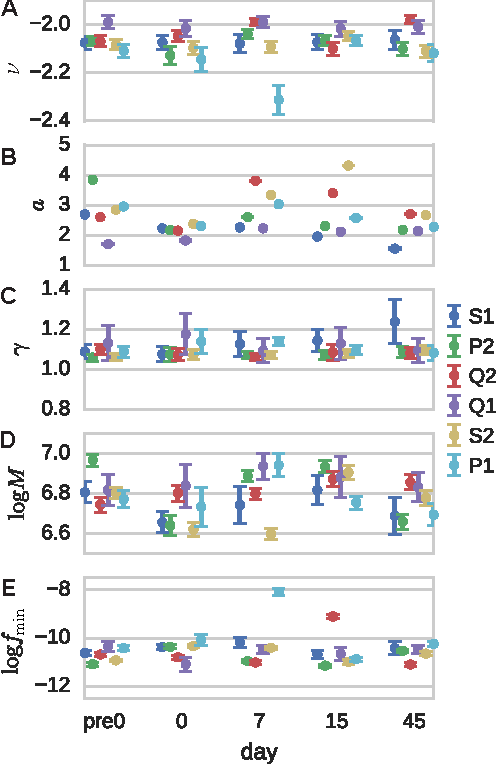
\includegraphics[width=.8\linewidth]{fig3_learnednullparas}
\centering{}
\caption{
  \emph{Inferred null model parameters}. Inferred values: for (A) the power-law exponent $\nu$ of the clone size distribution; (B) and (C) linear coefficient and exponent of the mean-variance relationship of the noise; (D) effective number of cells; and (E) minimal clonal frequency.
  Each point is inferred from a pair of replicates for a given donor and time point. Error bars are obtained by inverting the Hessian of the log-likelihood projected onto the hyperplane locally satisfying the normalization constraint.
\label{fig:nullparas_timeseries}}
\end{figure}


The inferred models can also be used to estimate the diversity of the entire repertoire (observed or unobserved).
The clone frequency distribution, $\rho(f)$, together with the estimate of $N$ can be used to estimate Hill diversities (see Methods):
\beq
D_\beta={\left(\sum_{i=1}^N f_i^\beta\right)}^{\frac{1}{1-\beta}}={\left(N\<f^\beta\>\right)}^{\frac{1}{1-\beta}}.
\eeq
In  \cref{fig:div_estimates}, we show the values, across donor and days, of three different diversities: species richness, i.e. the total number of clones $N$ ($\beta=0$); Shannon diversity, equal to the exponential of the Shannon entropy ($\beta=1$); and Simpson diversity, equal to the inverse probability that two cells belong to the same clone ($\beta=2$). In particular, estimates of $N\approx 10^9$ fall between the lower bound of $10^8$ unique TCRs reported in humans using extrapolation techniques \cite{Qi2014} and theoretical considerations giving upper-bound estimates of $10^{10}$ \cite{Lythe2016} or more \cite{Mora2019}.


\begin{figure}
%\includegraphics[width=\linewidth]{fig2_learnednullparas}
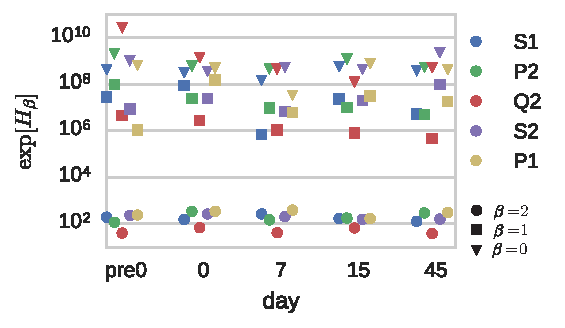
\includegraphics[width=\linewidth]{fig4_div_estimates}
\centering{}
\caption{\emph{Diversity estimates.} Shown are diversity estimates obtained from the Hill diversities, $D_\beta$, of the inferred clone frequency distributions for $\beta=0$ (estimated total number of clones, $N$), $\beta=1$ (Shannon entropy) and $\beta=2$ (Simpson index), across donors and days.
\label{fig:div_estimates}}
\end{figure}

